\documentclass{article}

\usepackage{graphicx}
\usepackage{tikz}
\usepackage{tikzsymbols}
\usetikzlibrary{calc,patterns,shapes.geometric}
\pagestyle{empty}
\usepackage[margin=0pt]{geometry}
\geometry{papersize={14in,12in}}

\def\centerarc[#1](#2)(#3:#4:#5){\draw[#1] ($(#2)+({#5*cos(#3)},{#5*sin(#3)})$) arc (#3:#4:#5);}

\begin{document}
	\begin{figure}
		\centering
		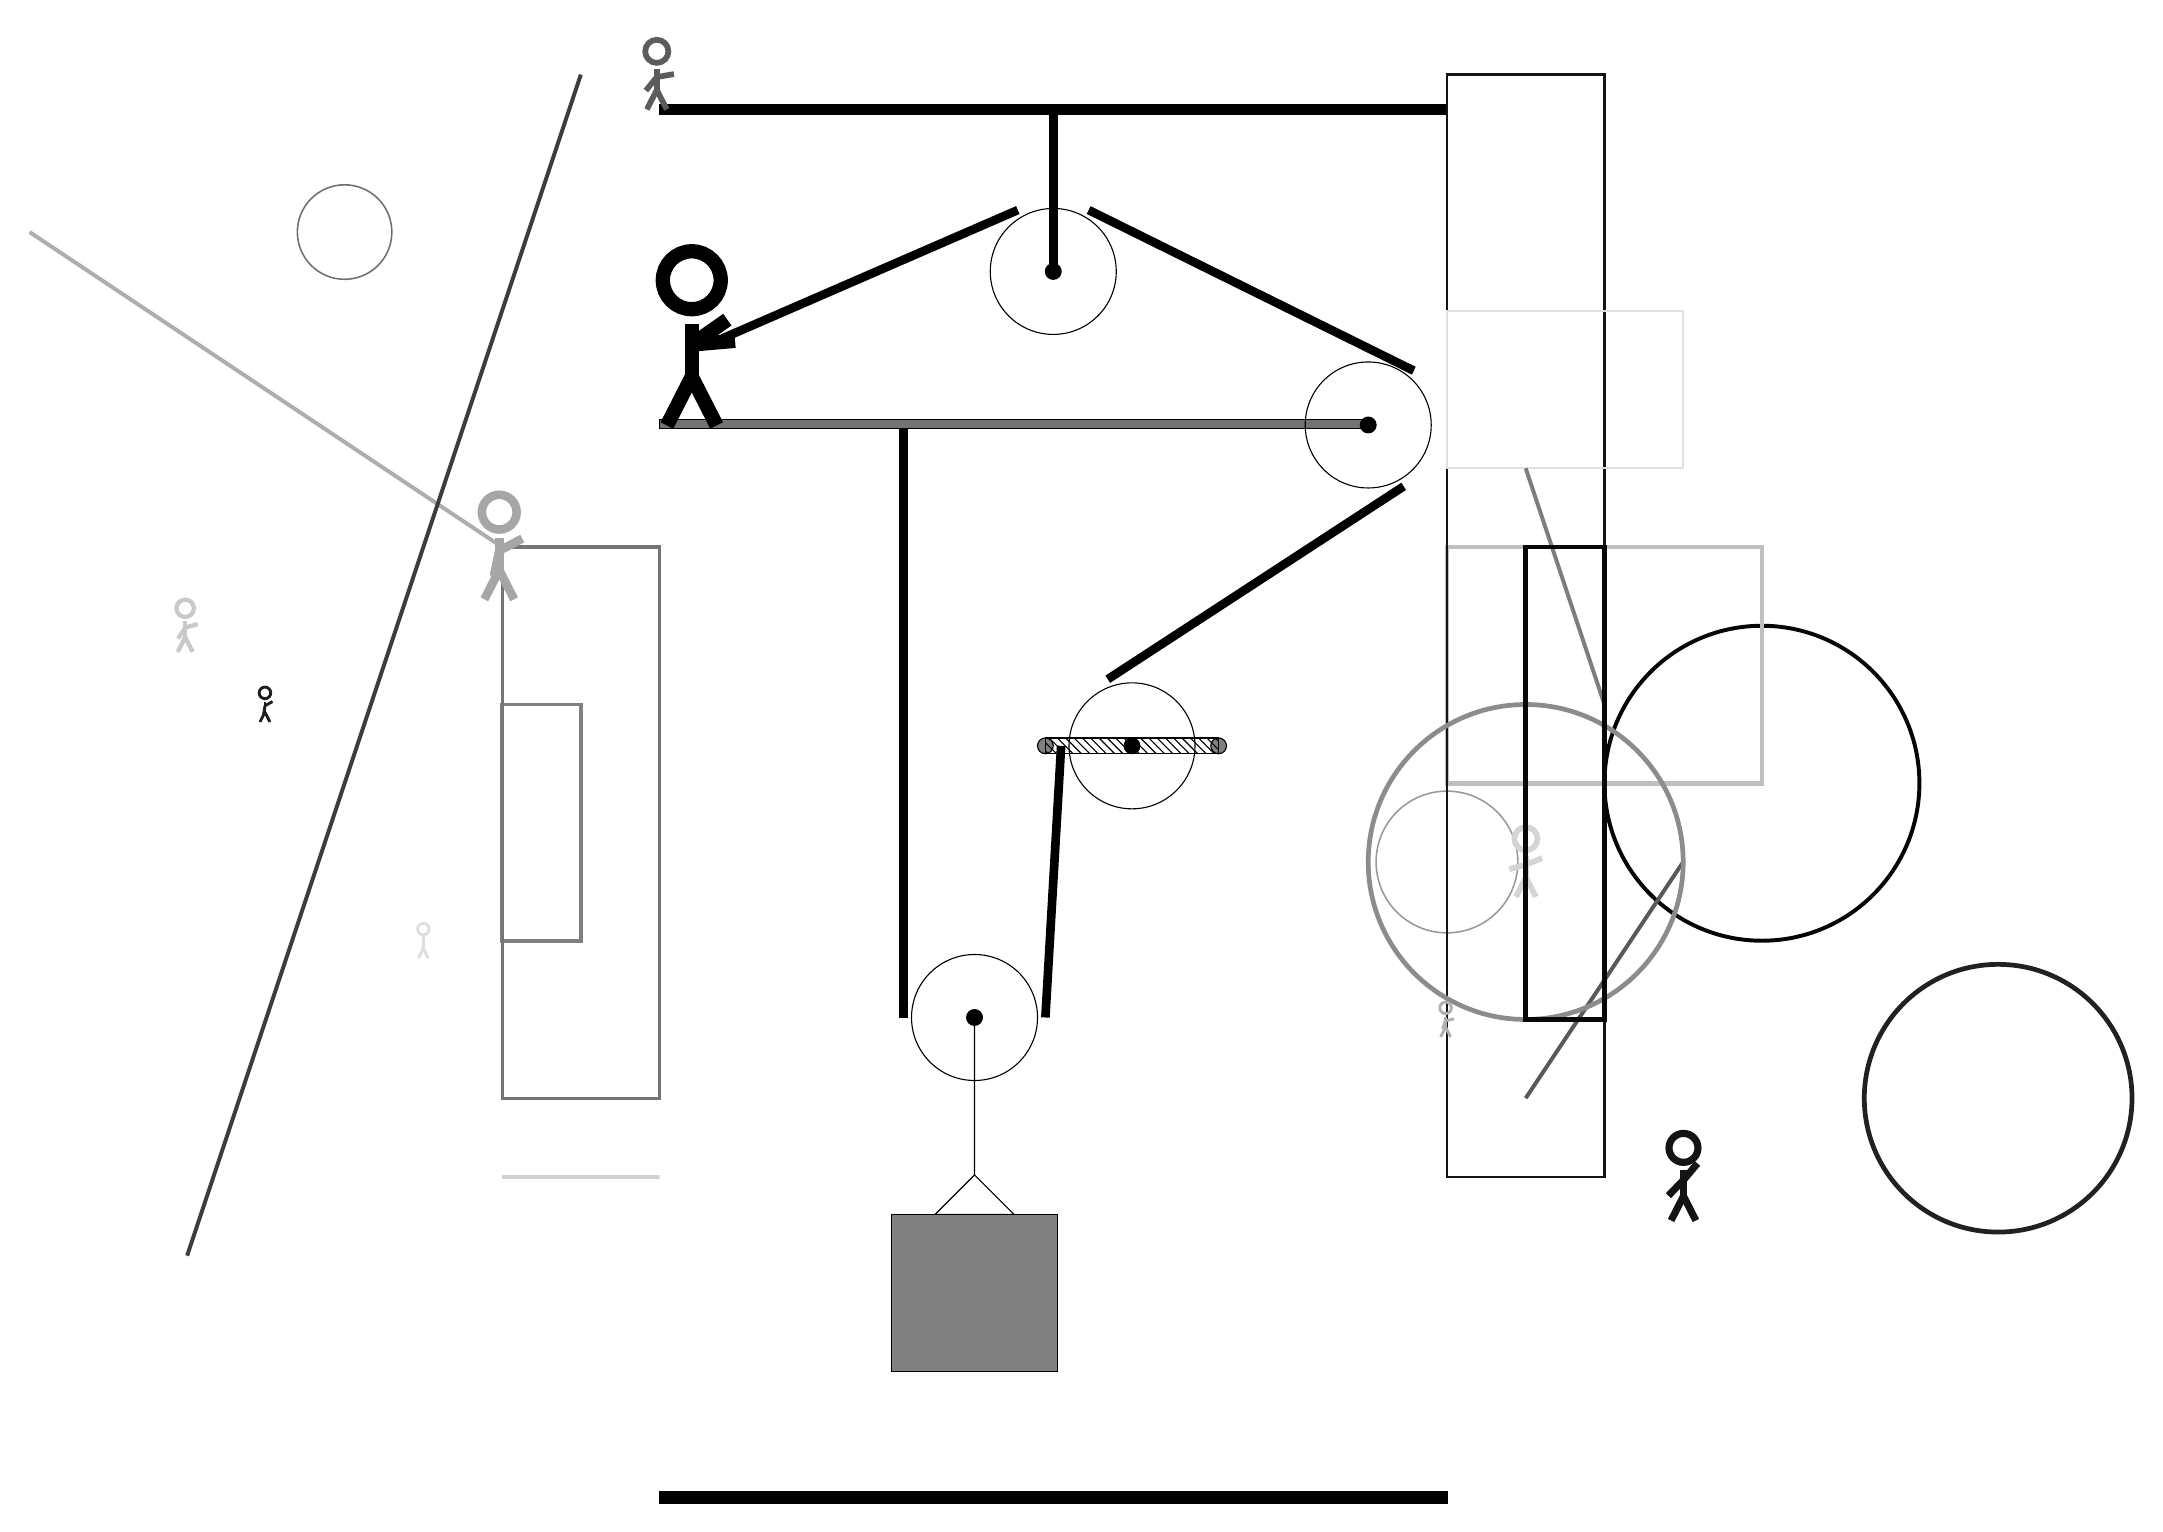
\begin{tikzpicture}
			%%%%% START %%%%%
			
			\draw[fill=black] (-2, 15.5) rectangle (8, 15.625);
			
			\draw[fill=black!55] (-2, 11.5) rectangle (7, 11.625);
			
			\draw (2, 4.025) circle (0.8);
			\draw[fill=black] (2, 4.025) circle (0.1);
			
			\draw (7, 11.55) circle (0.8);
			\draw[fill=black] (7, 11.55) circle (0.1);
			
			\draw[fill=white](4, 7.475) circle (0.8);
			\draw[fill=black] (4, 7.475) circle (0.1);
			\draw[fill=black!50] (2.9, 7.475) circle (0.1);
			\draw[fill=black!50] (5.1, 7.475) circle (0.1);
			\draw[pattern=north west lines, pattern color=black] (2.9, 7.575) rectangle (5.1, 7.375);
			
			\draw (3, 13.5) circle (0.8);
			\draw[fill=black] (3, 13.5) circle (0.1);
			\draw[line width=1.1mm] (3, 13.5) -- (3, 15.5);
			
			\draw [line width=0.5mm, color=black!98](12, 7) circle (2.0);
			
			\node[line width=0.6mm, color=black!21] at (-8, 9) {\Strichmaxerl[3][57][16]};
			\draw [line width=0.2mm, color=black!40](8, 6) circle (0.9);
			\node[line width=0.2mm, color=black!64] at (-2, 16) {\Strichmaxerl[4][51][10]};
			
			\draw[line width=0.6mm, color=black!25] (8, 10) rectangle (12, 7);
			
			\node[line width=0.7mm, color=black!13] at (-5, 5) {\Strichmaxerl[2][87][86]};
			
			\draw[line width=0.3mm, color=black!92] (8, 2) rectangle (10, 16);
			\draw[line width=0.5mm, color=black!65](11, 6) -- (9, 3);
			\draw[line width=0.5mm, color=black!32](-4, 10) -- (-10, 14);
			\node[line width=0.5mm, color=black!17] at (9, 6) {\Strichmaxerl[4][16][21]};
			\draw[line width=0.4mm, color=black!18] (-2, 2) rectangle (-4, 2);
			\draw [line width=0.6mm, color=black!45](9, 6) circle (2.0);
			\draw[line width=0.5mm, color=black!50] (-4, 5) rectangle (-3, 8);
			\draw[line width=0.4mm, color=black!54] (-4, 10) rectangle (-2, 3);
			\draw [line width=0.2mm, color=black!56](-6, 14) circle (0.6);
			\node[line width=0.6mm, color=black!35] at (-4, 10) {\Strichmaxerl[6][78][28]};
			
			\node[line width=0.4mm, color=black!31] at (8, 4) {\Strichmaxerl[2][69][12]};
			
			\draw[line width=0.2mm, color=black!12] (8, 13) rectangle (11, 11);
			\draw[line width=0.5mm, color=black!76](-3, 16) -- (-8, 1);
			
			\draw[line width=0.5mm, color=black!51](10, 8) -- (9, 11);
			\draw [line width=0.6mm, color=black!57](-2, 10) circle (0.0);
			
			\draw[line width=0.6mm, color=black!97] (10, 10) rectangle (9, 4);
			\node[line width=0.2mm, color=black!92] at (11, 2) {\Strichmaxerl[5][46][50]};
			\node[line width=0.2mm, color=black!88] at (-7, 8) {\Strichmaxerl[2][81][29]};
			\draw [line width=0.6mm, color=black!87](15, 3) circle (1.7);
			
			
			\draw (2, 4.025) -- (2, 2.025) -- (1.5, 1.525) -- (2.5, 1.525) -- (2, 2.025);
			\draw[fill=black!50] (0.95, 1.525) rectangle (3.05, -0.475);
			
			\draw[line width=1.1mm] (1.1, 11.5) -- (1.1, 4.025);
			\centerarc[line width=1.1mm](2, 4.025)(180:360:0.9);
			\draw[line width=1.1mm](2.9, 4.025) -- (3.1, 7.475);
			\centerarc[line width=1.1mm](4, 7.475)(110:180:0.9);
			\draw[line width=1.1mm](3.6922, 8.3207) -- (7.45, 10.7706);
			\centerarc[line width=1.1mm](7, 11.55)(-60:50:0.9);
			\draw[line width=1.1mm](7.5785, 12.2394) -- (3.45, 14.2794);
			\centerarc[line width=1.1mm](3, 13.5)(60:120:0.9);
			\draw[line width=1.1mm](2.55, 14.2794) -- (-1.2, 12.65);
			
			\node at (-1.5, 12.65) {\Strichmaxerl[10][-175][35]};
			
			\draw[fill=black] (-2, -2) rectangle (8, -2.15);
			
			%%%%% END %%%%%
		\end{tikzpicture}
	\end{figure}	
\end{document}